\documentclass[compress, 10pt]{beamer}
\usepackage{nuaabeamer}

\usepackage{graphics}

\usepackage{frame}
\usepackage{pgf}
\usepackage[UTF8, noindent]{ctex}
\usepackage{times}
\usepackage{amsmath}
\usefonttheme{professionalfonts}

\usepackage{caption}
\setbeamertemplate{caption}[numbered]{}

\usepackage[backend=bibtex,style=ieee,sorting=none]{biblatex}
\addbibresource{ref.bib}
\setbeamerfont{footnote}{size=\tiny}

\usepackage{subfigure}

\makeatletter
\let\@@magyar@captionfix\relax
\makeatother

\newcommand{\Title}{SPH方法调研与汇报一}
\newcommand{\Reporter}{包晨宇}
\newcommand{\Instructor}{吕宏强}
\newcommand{\Institute}{南京航空航天大学}

\begin{document}

\captionsetup[figure]{font=footnotesize,labelfont=footnotesize}

\title{\Title}
\author{汇报人:\Reporter \\ \vspace{1em} 指导人:\Instructor}
\date{\today}
\institute{\Institute}

\begin{frame}
    \begin{figure}[H]
        \centering
        
\includegraphics[width=0.2\textwidth]{logo.pdf}
    \end{figure}
    \maketitle
\end{frame}

\section*{目录}
\begin{frame}
    \frametitle{\secname}
    \tableofcontents[sections={<1-5>}]
\end{frame}

\AtBeginSection[] {%在每一节前面加入目录显示当前节的目录结构
	\begin{frame}
		\frametitle{目录}
		\tableofcontents[currentsection,currentsubsection,hideothersubsections,sectionstyle=show/shaded,]
		\addtocounter{framenumber}{-1}  %目录页不计入页码
	\end{frame}
}

\section{SPH方法简介}

\subsection{发展历程}

\begin{frame}
    \begin{itemize}
		\item 光滑粒子流体动力学(Smoothed Particle Hydrodynamics,SPH)
		方法是一种基于拉格朗日方法的流体数值模拟方法,
		由英国物理学家Lucy于1977年首次提出,Gingold和Monaghan于1977年独立提出,
		1985年Monaghan发表了SPH方法的第一篇综述性论文,SPH方法自此开始快速发展。

		\item 作为一种无网格方法(meshfree)方法,
		SPH方法并非真的不需要网格,而是求解精度不那么依赖于网格的结构。
	
		\item SPH方法通过大量粒子来离散研究对象,
	    每一个粒子代表该对象中的介质团,粒子之间无直接的网格联系,
		因此可以有效地避免传统网格方法难以处理的网格畸变问题。
	
		\item 最初的SPH方法是用于求解天体物理问题的,后来被应用于流体动力学、
		固体力学、热力学、电磁学、生物力学、地质力学等。
	\end{itemize}
\end{frame}

\begin{frame}
	SPH方法更多地还是被应用在水动力学领域
	(因其数值特性和精度问题,在气动分析中应用受到限制)。

	SPH方法有多种形式,主要有两类形式\cite{_sph_2022}:
	\begin{itemize}
		\item 不可压SPH方法(Incompressible SPH,ISPH)
		\item 弱可压SPH方法(Weakly Compressible SPH,WCSPH),
		由Monaghan于1994年引入,便于求解压力;
		而Shadloo等人验证了WCSPH方法在求解低雷诺数时翼型绕流的有效性。
	\end{itemize}

	相对而言,
	WCSPH相关理论和方法经过近20年的发展,
	计算精度已得到 明显提高,
	相比于ISPH方法,WCSPH方法涉及的GPU存储量更小,
	计算效率更高,所以更适合于开源程序的设计。
	DualSPHysics、SPHinXsys等开源程序包都是基于WCSPH理论框架的。
\end{frame}

\subsection{应用场景}

\begin{frame}
	SPH常用的应用场景有:
	\begin{itemize}
		\item 水下爆炸冲击波传播,如水下爆炸冲击波对船体的冲击;
		\item 水面波浪传播,如海洋中的海浪、风浪、涌浪等;
		\item 海岸、河流、湖泊等水体的水动力学过程,如水流泥沙、悬浮物等;
		\item 固体边界存在大变形的流固耦合问题;
		\item 生物医学领域,此时会涉及到多相流、多组分流、多物理场耦合等问题;
	\end{itemize}
\end{frame}
\section{SPH方法数学基础}

\subsection{$\delta$ 函数与光滑函数}

\begin{frame}
    $\delta$ 函数是一个由积分性质定义的特殊函数,在一维情况下其定义为:
    \begin{equation}
        \begin{aligned}
            &\delta(x) = \begin{cases}
                +\infty, & x = 0 \\
                0, & x \neq 0
            \end{cases}
            \\
            &\int_{-\infty}^{+\infty} \delta(x) \mathrm{d}x = 1
        \end{aligned}
    \end{equation}

    其具有两个重要的性质:

    \begin{itemize}
        \item 紧致性:$\delta(x) = 0, \forall x \neq 0$
        \item 筛选性:$\int_{-\infty}^{+\infty} f(\xi) \delta(x - \xi) \mathrm{d}\xi = f(x)$
    \end{itemize}

    上述两个性质是SPH方法产生的数学基础,
    根据紧致性和筛选性质,
    我们可以根据 $\delta$ 函数的这两个性质构造一个与之类似的光滑函数(或者称核函数) $W(x;h)$ ,
    其应该满足:
    \begin{equation}
        \begin{aligned}
            &W(x;h) = 0, \forall |x| > th\\
            &\int_{-\infty}^{+\infty} W(x;h) \mathrm{d}x = 1
        \end{aligned}
    \end{equation}
\end{frame}

\begin{frame}
    这里给出一个核函数的例子:
    \begin{equation}
        W(\vec{r};h) = \begin{cases}
            \frac{315}{64\pi h^9} (h^2 - |\vec{r}|^2)^3, & 0 \leq |\vec{r}| \leq h \\
            0, & |\vec{r}| > h
        \end{cases}
    \end{equation}

    \begin{figure}[H]
        \centering
        \subfigure[$\delta(x)$ 函数]{
            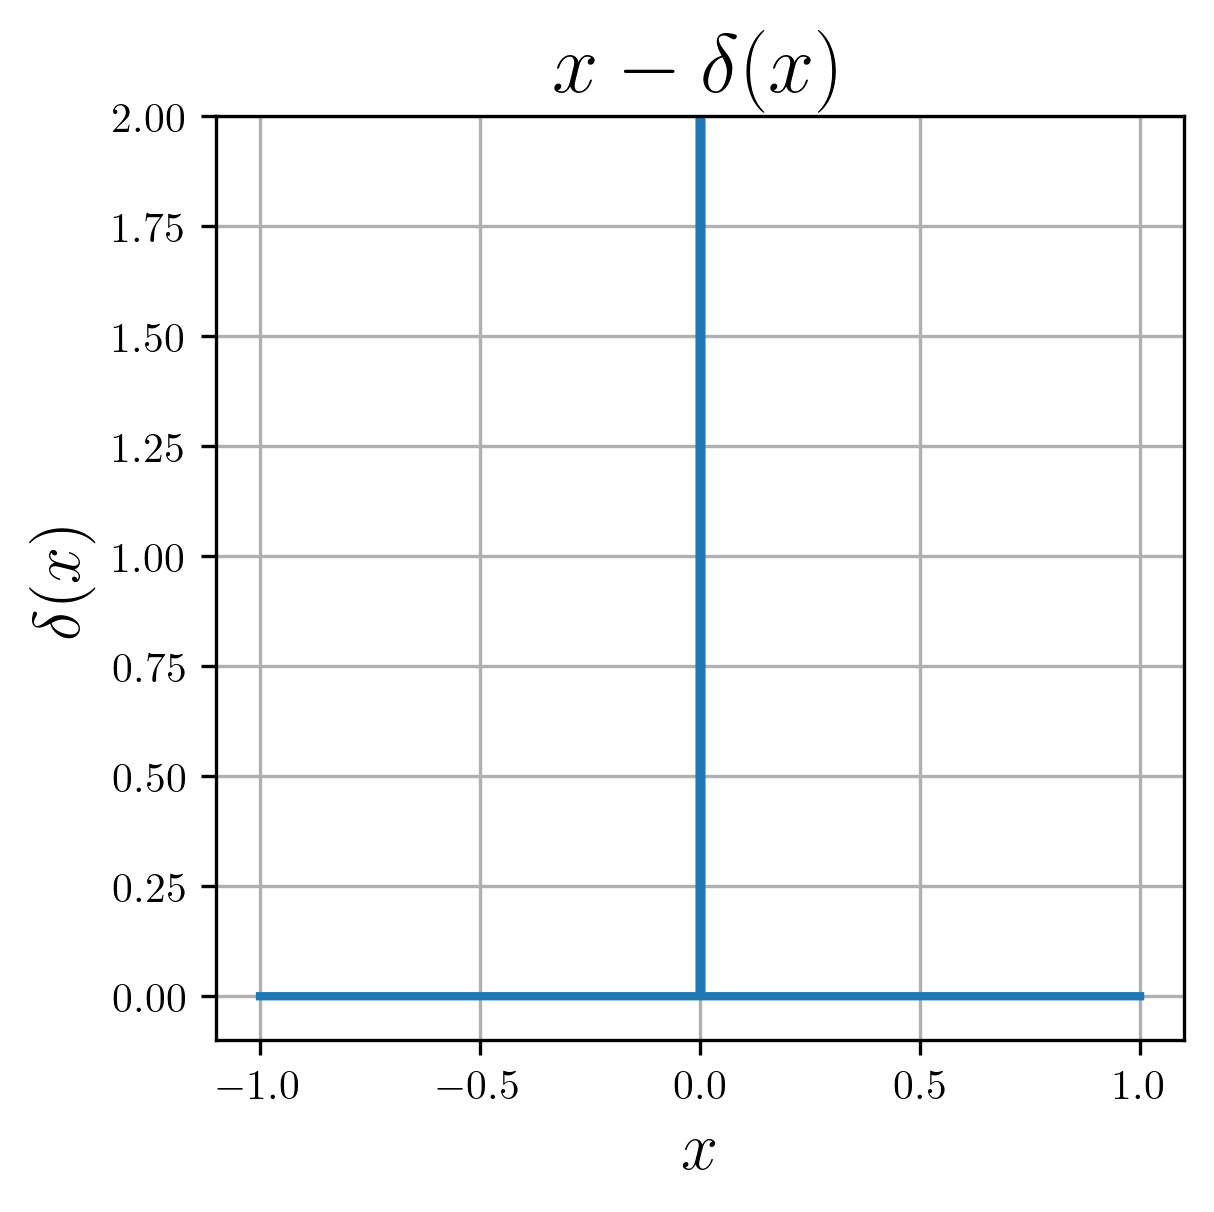
\includegraphics[width=0.3\textwidth]{images/delta.png}
        }
        \qquad
        \subfigure[光滑核函数(一维剖面)]{
            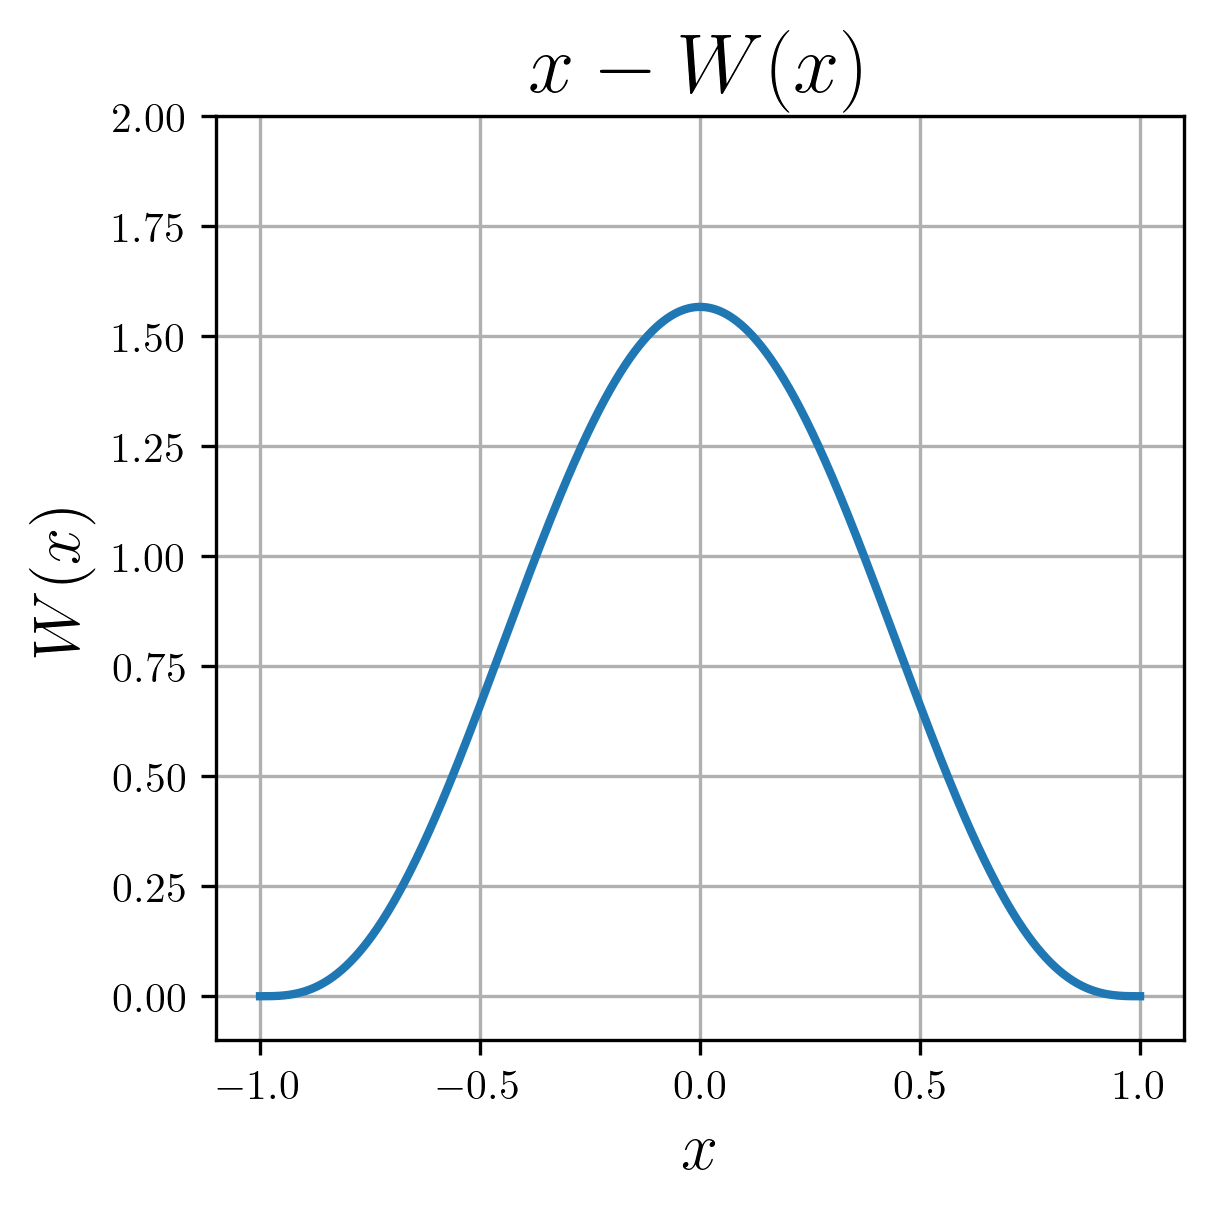
\includegraphics[width=0.3\textwidth]{images/W.png}
        }
        \caption{$\delta$ 函数与光滑核函数的示意图}
    \end{figure}

    这里需要补充说明的是,在编程实践中 $h$ 表示核半径,
    $t$ 表示核半径的某个倍数,数学推导中取 $t = 1$ 。
\end{frame}

\begin{frame}
    根据 $\delta$ 函数的两个性质,我们可以用 $W$ 光滑函数导出如下两个近似:

    \begin{itemize}
        \item 筛选性:
        \begin{equation}
            u(\vec{r})\approx \int_{\Omega} u(\vec{r}^\prime) 
            W(\vec{r} - \vec{r}^\prime;h) \mathrm{d}\vec{r}^\prime
        \end{equation}
        \item 紧致性:
        \begin{equation}
            \begin{aligned}
                \nabla u(\vec{r}) &\approx \int_{\Omega} \nabla u(\vec{r}^\prime)
                W(\vec{r} - \vec{r}^\prime;h) \mathrm{d}\vec{r}^\prime \\
                &=
                \int_{\partial\Omega} u(\vec{r}^\prime) \vec{n}(\vec{r}^\prime)
                W(\vec{r} - \vec{r}^\prime;h) \mathrm{d}S^\prime - 
                \int_{\Omega} u(\vec{r}^\prime) \nabla^\prime
                W(\vec{r} - \vec{r}^\prime;h) \mathrm{d}\vec{r}^\prime\\
                &\mathop{=}^{\text{紧致性}} -\int_{\Omega} u(\vec{r}^\prime) \nabla^\prime
                W(\vec{r} - \vec{r}^\prime;h) \mathrm{d}\vec{r}^\prime
            \end{aligned}
        \end{equation}
    \end{itemize}

    上述两个式子是SPH方法的数学基础,表明某个标量场 $u(\vec{r})$ 
    和其在该点的梯度 $\nabla u(\vec{r})$ 可以用该点附近的标量场值在光滑核函数加权下的积分来近似。
\end{frame}

\subsection{物质点的离散}

\begin{frame}
    我们先考虑标量场 $u(\vec{r})$ 值的近似,假设我们有 $N$ 个物质点,
    任意分布在 $\Omega$ 区域内,其位置分别为 $\vec{r}_i, i = 1, 2, \cdots, N$ ,
    则标量场 $u(\vec{r})$ 在 $\vec{r}_i$ 处的近似值为:
    \begin{equation}
        \label{eq:scalar_field_approximation}
        \begin{aligned}
            u(\vec{r})&\approx \int_{\Omega} u(\vec{r}^\prime) 
                W(\vec{r} - \vec{r}^\prime;h) \mathrm{d}\vec{r}^\prime\\
            &\approx
            \sum_{j=1}^{N} u_j W(\vec{r} - \vec{r}_j;h) V_j\\
            &=
            \sum_{j=1}^{N} u_j W(\vec{r} - \vec{r}_j;h) \frac{m_j}{\rho_j}
        \end{aligned}
    \end{equation}

    为方便起见,我们认为质点 $j$ 的体积 $V_j$ 由该质点携带的质量与其密度之比得到。
    考虑质点 $k$ 处的值,可以将上述表达式写成:
    \begin{equation}
        u_k = \sum_{j=1}^{N} u_j W_{kj} \frac{m_j}{\rho_j}
    \end{equation}
\end{frame}

\begin{frame}
    \begin{figure}[H]
        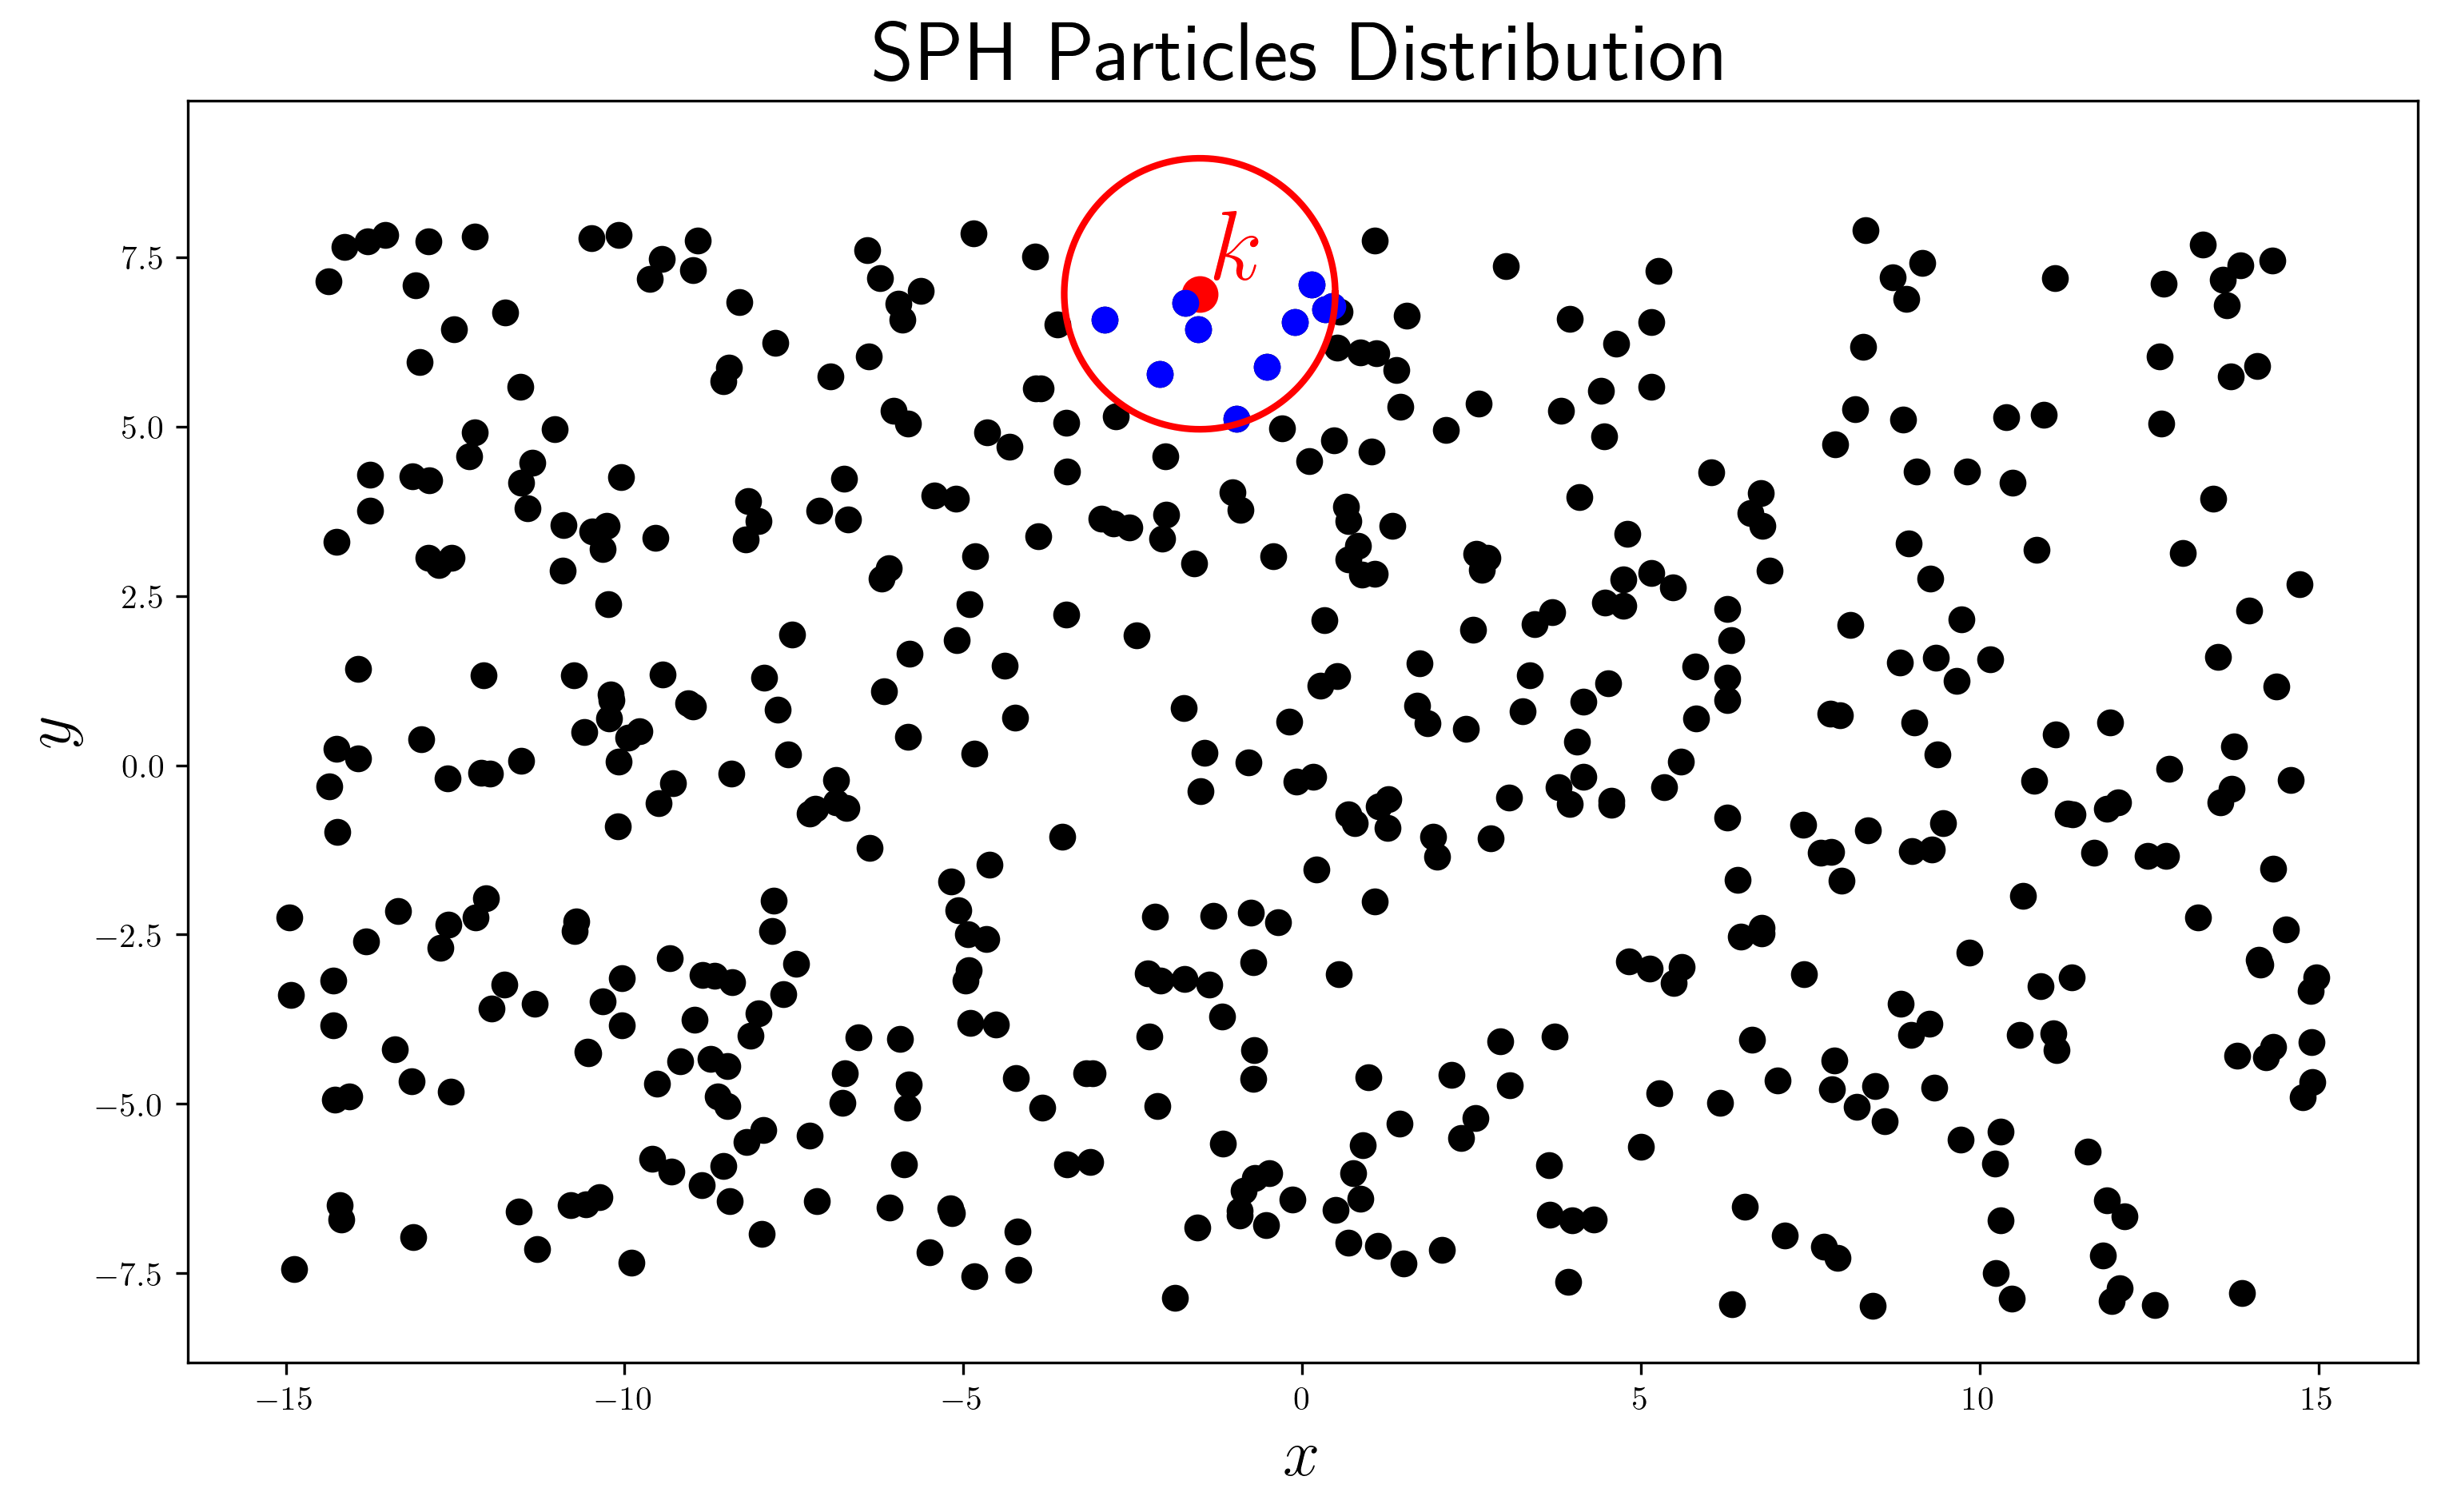
\includegraphics[width=0.7\textwidth]{images/sph_particles_distribution.png}
        \caption{物质点分布示意图}
        \label{fig:particles_distribution}
    \end{figure}
    而因为紧致性,事实上并不是所有的质点都会对质点 $k$ 处的值产生影响,
    仅在其核半径球内的质点才会对其产生影响,如图 \ref{fig:particles_distribution} 所示,
    编程中常用Hash表来存储这些质点,以加快计算速度。
    当然式 \ref{eq:scalar_field_approximation} 中的积分也有其他的格式,
    类似于传统FVM中的数值格式。
\end{frame}

\begin{frame}
    \begin{block}{各种格式的标量梯度的核函数插值}
        \begin{equation}
            \begin{aligned}
                \nabla u(\vec{r}_i) &= 
                    \sum_{j=1}^N
                    \frac{m_j}{\rho_j} u(\vec{r}_j)\frac{\vec{r}_i-\vec{r}_j}{r_{ij}}
                    \frac{\partial W_{ij}}{\partial r_{ij}}\\
                \nabla u(\vec{r}_i) &=
                    \frac{1}{\rho_i}\sum_{j=1}^N m_j [u(\vec{r}_j) - u(\vec{r}_i)]
                    \frac{\vec{r}_i-\vec{r}_j}{r_{ij}}\frac{\partial W_{ij}}{\partial r_{ij}}\\
                \nabla u(\vec{r}_i) &= \rho_i
                    \sum_{j=1}^N \frac{m_j}{\rho_j^2} 
                    \left[
                        \frac{u(\vec{r}_j)}{\rho_j^2} + \frac{u(\vec{r}_i)}{\rho_i^2}
                    \right]
                    \frac{\vec{r}_i-\vec{r}_j}{r_{ij}}\frac{\partial W_{ij}}{\partial r_{ij}}\\
            \end{aligned}
        \end{equation}
    \end{block}
\end{frame}

\subsection{控制方程和算法流程}

\begin{frame}
    在给出方程前首先需要注意的事情是SPH方法是基于拉格朗日描述的,
    对于不可压流体(一般用来求解不可压问题),
    Kochier与Bender \cite{koschier_smoothed_2020} 给出控制方程如下:
    \begin{equation}
        \begin{cases}
            &\nabla\cdot\vec{u} = 0\\
            &\rho \frac{\partial \vec{u}}{\partial t} = 
            -\nabla p + \mu \nabla^2 \vec{u} + \vec{f}
        \end{cases}
    \end{equation}
    他们给出了一套较为完整的算法流程,大致如下:
    \begin{itemize}
        \item 对所有粒子求解 $\frac{\partial \vec{u}}{\partial t}=\nu\nabla^2\vec{u}+\frac{1}{\rho}\vec{f}$ ;
        \item 根据不可压性质,求解 $\nabla p=\vec{0}$ ;
        \item 再次更新速度场 $\frac{\partial \vec{u}}{\partial t}=-\frac{1}{\rho}\nabla p$ ;
        \item 更新所有粒子位置 $\vec{x}_{\text{next}}=\vec{x}_{\text{curr}}+\vec{u}\Delta t$ 。
    \end{itemize}
\end{frame}

\begin{frame}
    \begin{figure}[H]
        \centering
        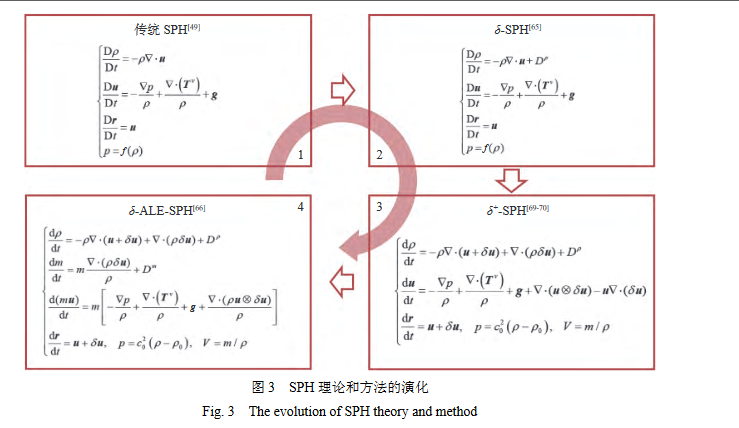
\includegraphics[width=0.8\textwidth]{images/sph离散方程.png}
        \caption{SPH方程离散形式的演化\cite{_sph_2022}}
    \end{figure}
    其中西工大黄晓婷\cite{_sph_2022-3}采用 $\delta^+$ SPH 方法求解翼型绕流问题。
    上述过程虽然看起来比较简单
    但实际在计算的过程中会涉及到很多问题,
    依目前查询文献结果来看,
    可能遇到的问题如下如质点质量分布的初始化\cite{tian_systematic_2017},
    自由表面捕捉问题\cite{_sph_2022-1},
    压力梯度精度不足导致的数值空腔\cite{_sph_2022-3}等。
\end{frame}

\subsection{边界条件的处理}

\begin{frame}
    SPH方法的边界条件处理是一个比较复杂的问题,
    一般来说,边界条件可以分为两类:自由边界和固壁边界。
    \begin{block}{自由边界}
        采用追踪法,即在计算过程中,
        将自由表面的粒子标记出来,然后在计算过程中,
        通过求解自由表面的法向加速度来更新自由表面的位置。
        这块在蒋肖蒙\cite{_sph_2022-1}的硕士毕业论文钟有描述,
        其构建了一套自由表面捕捉和重构的方法。
    \end{block}
    \begin{block}{固壁边界}
        一般镜像法,即在计算过程中,
        将固壁边界的粒子标记出来,然后在计算过程中,
        通过求解固壁边界的法向加速度来更新固壁边界的位置,
        但这种方法需要进行压力修正以避免粒子堆积。
        另外还有固定虚粒子法和改进固定虚粒子法,
        即用固定的假想粒子来代替固壁边界。
    \end{block}
\end{frame}

\begin{frame}
    \begin{figure}[H]
        \subfigure[自由表面捕捉与重构]{
            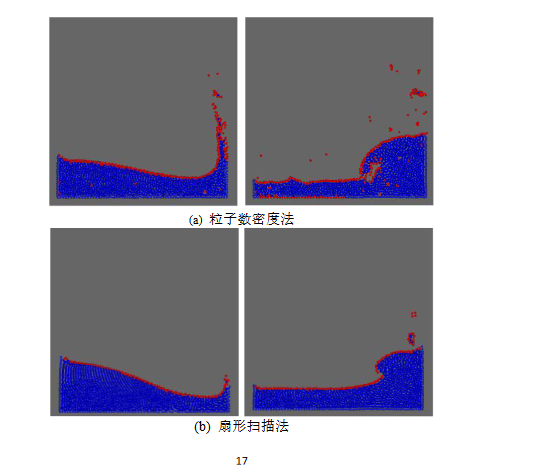
\includegraphics[width=0.42\textwidth]{images/surface_reconstruct.png}
        }
        \subfigure[固定边界虚粒子处理法]{
            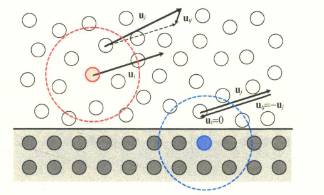
\includegraphics[width=0.52\textwidth]{images/fixed_bd.png}
        }
        \caption{两类常用边界处理方法}
    \end{figure}
\end{frame}
\section{SPH方法算例}

\subsection{文献中的算例}

\begin{frame}
    \begin{figure}[H]
        \centering
        \subfigure[水面兴波]{
            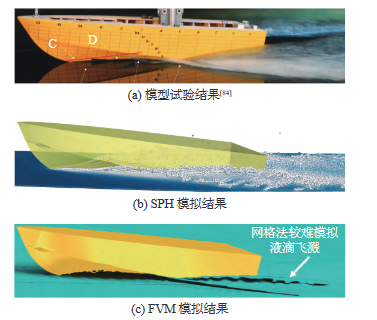
\includegraphics[width=0.3\textwidth]{images/xingbo.png}
        }
        \subfigure[细长体入水]{
            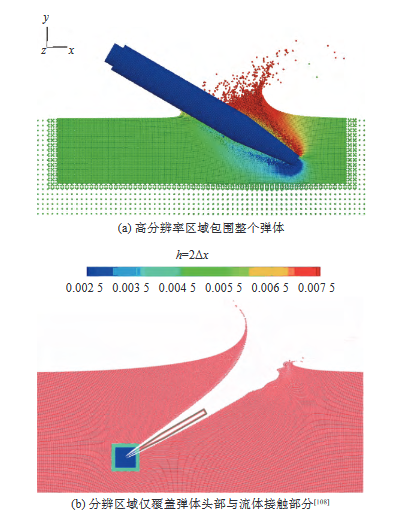
\includegraphics[width=0.25\textwidth]{images/xichangti.png}
        }\\
        \subfigure[水下爆炸]{
            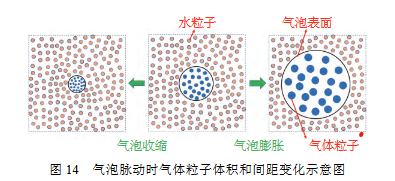
\includegraphics[width=0.5\textwidth]{images/shuixiabaozha.png}
        }
        \caption{SPH理论和方法在高速水动力学中的研究进展\cite{_sph_2022}}
    \end{figure}
\end{frame}

\begin{frame}
    \begin{figure}[H]
        \centering
        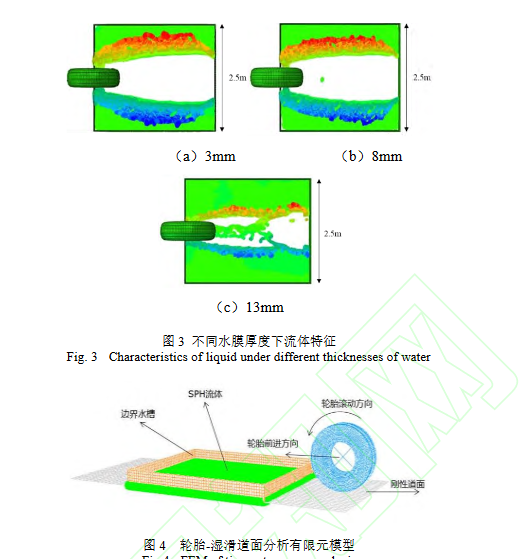
\includegraphics[width=0.6\textwidth]{images//luntai.png}
        \caption{飞机轮胎-湿滑道面相互作用SPH算法仿真分析\cite{_-sph_nodate}}
    \end{figure}
\end{frame}

\begin{frame}
        \begin{figure}[H]
            \centering
            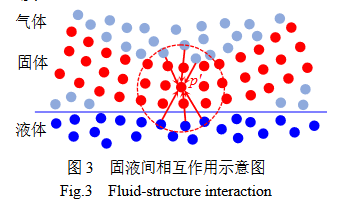
\includegraphics[width=0.6\textwidth]{images//tansuxing.png}
            \caption{基于改进光滑粒子流体动力学方法的弹塑性结构入水问题研究\cite{__nodate}}
        \end{figure}
\end{frame}

\begin{frame}
    \begin{figure}[H]
        \centering
        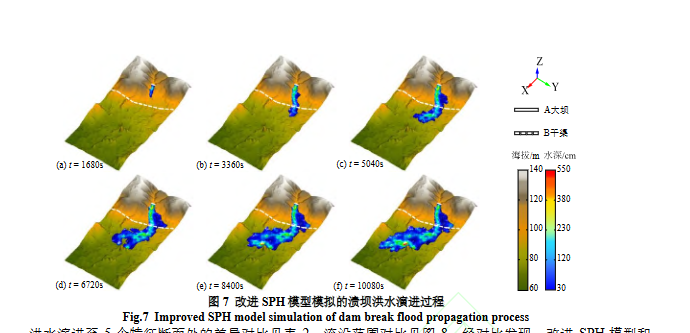
\includegraphics[width=0.6\textwidth]{images//kuibahongshui.png}
        \caption{基于改进SPH模型的溃坝洪水演进模拟方法\cite{_sph_nodate-2}}
    \end{figure}
\end{frame}

\begin{frame}
    \begin{figure}[H]
        \centering
        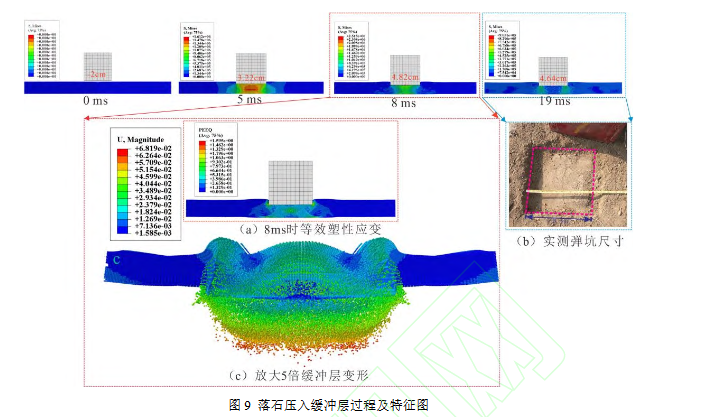
\includegraphics[width=0.6\textwidth]{images//ouhedabianxing.png}
        \caption{基于SPH-FEM的落石冲击缓冲层-钢筋混凝土板动力响应研究\cite{_sph-fem-_nodate}}
    \end{figure}
\end{frame}

\begin{frame}
    \begin{figure}[H]
        \centering
        \subfigure[粒子修正技术]{
            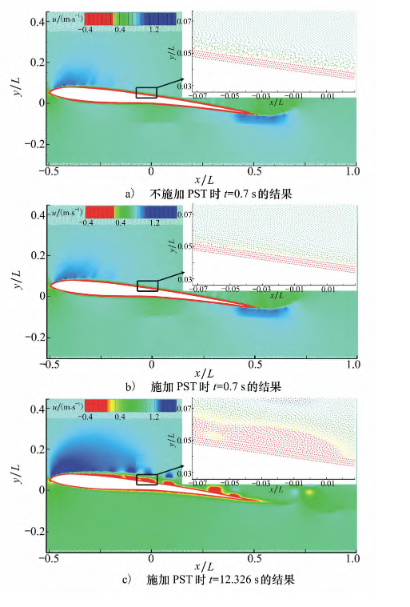
\includegraphics[width=0.2\textwidth]{images/lizixiuzheng.png}
        }\quad
        \subfigure[张力不稳定控制]{
            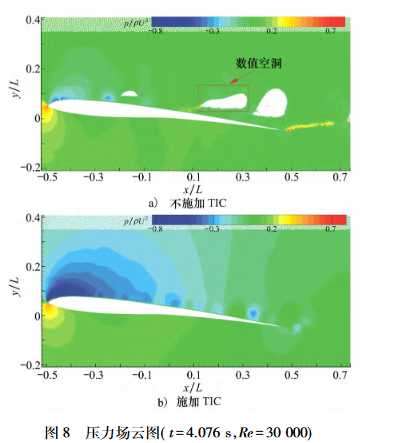
\includegraphics[width=0.25\textwidth]{images/zhanglibuwendingkongzhi.png}
        }\quad
        \subfigure[多级粒子分辨率技术与拉格朗日拟序结构]{
            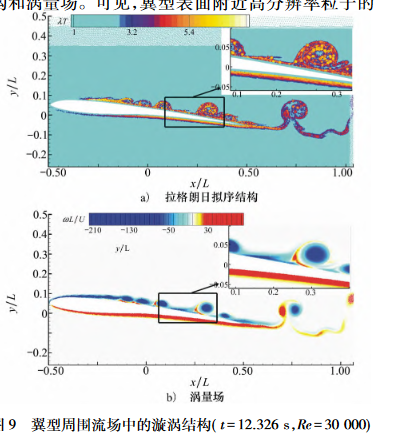
\includegraphics[width=0.25\textwidth]{images/duojilizi.png}
        }
        \caption{翼型绕流的多级分辨率光滑粒子流体动力学数值模拟研究\cite{__2022-3}}
    \end{figure}
\end{frame}

\subsection{SmoothedParticles.jl开源库算例}

\begin{frame}
    SmoothedParticles.jl是一个基于Julia语言的开源并行SPH库,
    其以Julia语言的高性能为基础,实现了SPH方法的核心算法,
    并将结果以Paraview的格式输出,方便后续的后处理。
    \begin{figure}[H]
        \centering
        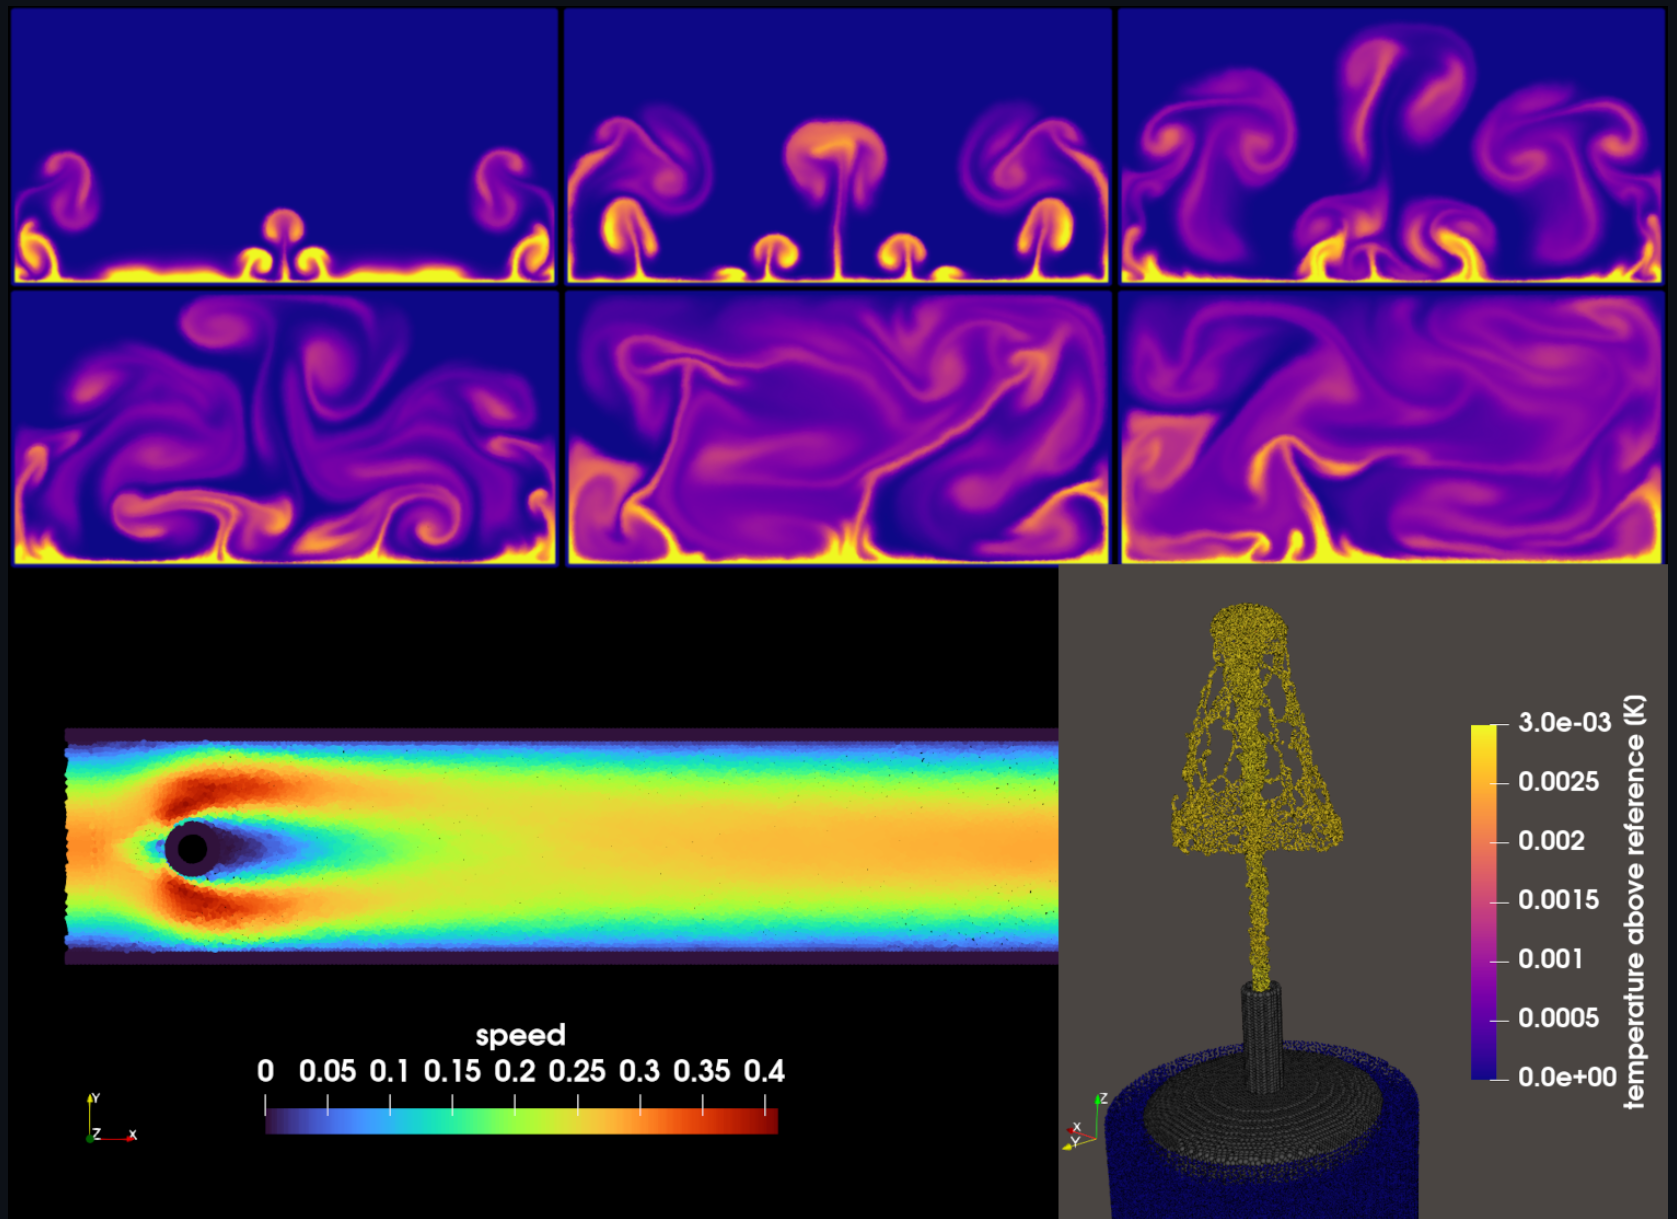
\includegraphics[width=0.6\textwidth]{images/smoothedparticles.png}
        \caption{SmoothedParticles.jl开源库}
    \end{figure}
\end{frame}

\begin{frame}

    \begin{figure}[H]
        \centering
        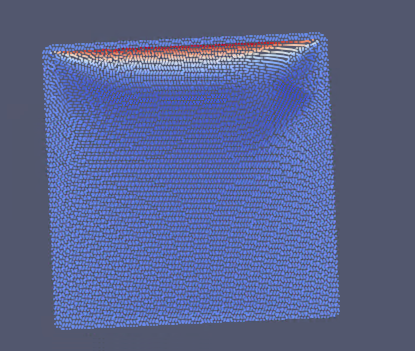
\includegraphics[width=0.6\textwidth]{images/lid_driven_cavity.png}
        \caption{顶盖驱动流算例}
    \end{figure}
\end{frame}

\begin{frame}
    \begin{figure}[H]
        \centering
        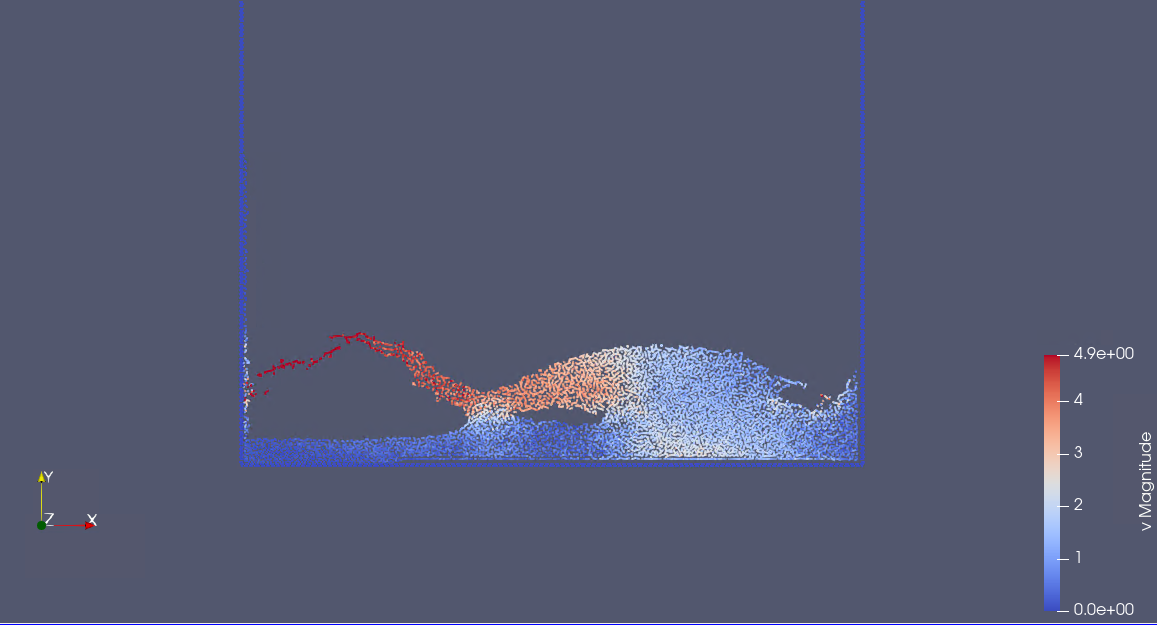
\includegraphics[width=0.6\textwidth]{images/free_surface.png}
        \caption{自由表面流}
    \end{figure}
    此算例用显示时间推进,计算了3000个粒子的运动,花费了40分钟。
\end{frame}

\begin{frame}
    \begin{figure}[H]
        \centering
        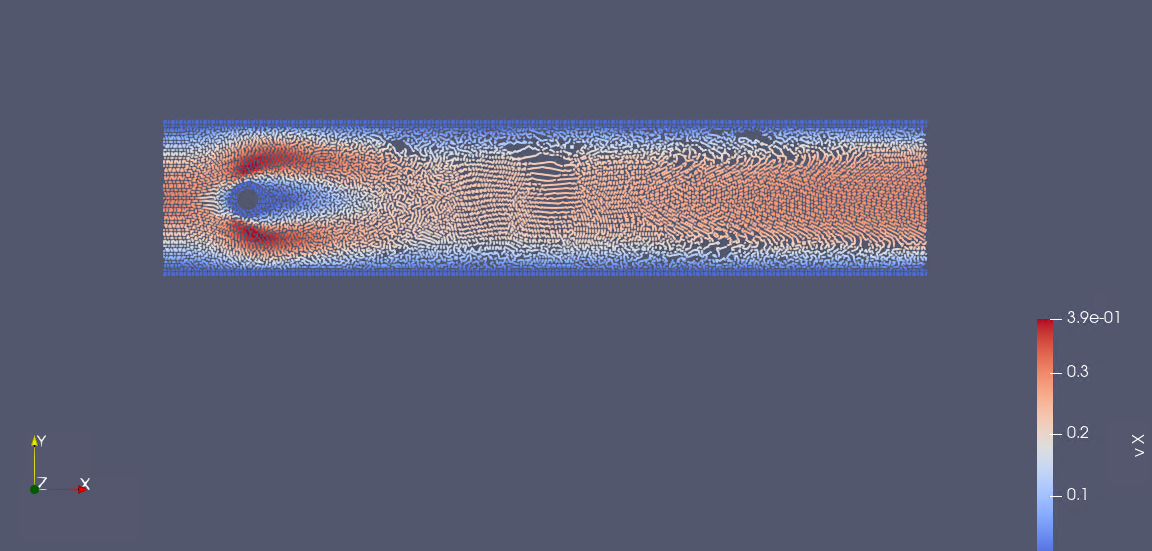
\includegraphics[width=0.6\textwidth]{images/cylindar.png}
        \caption{圆柱绕流}
    \end{figure}
\end{frame}
\section{SPH方法总结}


\subsection{SPH方法思想总结}

\begin{frame}
\begin{block}{一个比喻}
    在我简单的学习和阅读文献后,
    我认为SPH方法可以用一个形象的比喻来描述:
    假想我们在流体内细密地分布一种可以吸附流体的“吸水珠”,
    可以将附近核半径内的流体吸附到自己体内,
    形成一个理想质点。

    这样做的好处是,
    在求解方程时,
    这些吸水珠同时有如下两种性质:
    \begin{itemize}
        \item 质点性质:涉及到拉格朗日描述下刚体运动求解时,
        吸水珠呈现出质点的性质,即质点的质量、速度、位置等,
        此时流体质量都集中在这个质点上;
        \item 连续介质性质:在涉及到流体运动求解时,
        需要用到速度场的空间导数,用光滑核函数把这个吸水珠打开,
        将质量、能量、动量平摊在附近的空间上,
        此时这个质点呈现出连续介质的特性。
    \end{itemize}

    在传统流体求解中,
    流体网格的粗细对求解结果精度有很大影响,
    网格越粗,精度越低,但求解越快。
    同样的,SPH方法中,
    光滑核函数半径越大,精度越低,流体分布越稀疏,但求解更快。

    而因为SPH方法中对流体质点间并没有建立明确的几何拓扑关系,
    所以这些质点往往可以自由移动,
    从而可以很好地模拟流体的自由表面,
    避免传统方法中网格畸变或者重构网格的复杂过程。
\end{block}
\end{frame}

\subsection{SPH方法优缺点总结}

\begin{frame}

    SPH方法优点:
    \begin{itemize}
        \item 适用于自由表面流动
        \item 适用于高速撞击流动,不需要网格加密
        \item 适用于多相流动,用于解决流动中的相变问题
        \item 适用于流动中的破碎问题
        \item 适用于流动中的边界大变形问题
    \end{itemize}

    SPH方法缺点:
    \begin{itemize}
        \item 计算效率低,计算量大(没有连接信息,每步都需要计算两点间距)
        \item 很难评估算法的精度与收敛性,且各类光滑核函数的选取缺乏数学理论支撑
        \item 在某些情况下会出现数值空腔,或者粒子堆积现象
        \item 其流动后处理(如计算压力、速度场等)较为困难
        \item 若要与其他方法结合,缺乏边界处物理场信息交换的方法
    \end{itemize}

\end{frame}

\section*{参考文献}
\begin{frame}[allowframebreaks]
	\frametitle{\secname}
	\printbibliography[heading=none]
\end{frame}

\end{document}